%% ============================================================
%% Breaking the Bubble? — PNAS DRAFT (August 2026)
%%
%% Derived from DisasterAIFilter_NHB.tex following
%% PNAS_WRITING_INSTRUCTIONS.md. Changes from the NHB draft:
%%
%%  * Format: PNAS genre — Significance Statement (<=120 w),
%%    abstract <=250 w, ~4,000-4,500 words main text, 4 display
%%    items (all figures; every table is SI), Materials & Methods
%%    as the final main-text section, American English.
%%    SUBMISSION: swap \documentclass to pnas-new.cls. The file is
%%    kept sn-jnl-compilable during drafting.
%%  * Metric revision (M1): the AI-side echo construct is now
%%    AECI-IE — SECI's own variance-ratio construct applied to the
%%    report levels a channel SERVES a community — with SECI-IE as
%%    its human-channel consistency check and AECI-IE-rel (served
%%    pool vs the community's OWN beliefs) as the mirror index.
%%    AECI-Var is retired to the alpha* sensitivity table (Table S2).
%%  * The AI is type-agnostic: it targets the caller's own revealed
%%    prior for BOTH agent types. The "consensus recycling"
%%    mechanism of the NHB draft is deleted throughout (it described
%%    legacy code and the ablation shows the targeting is inert).
%%  * Per-type reporting is the default for SECI, MAE, AECI-IE,
%%    trust and query shares.
%%
%% NUMBERS. Existing metrics: run 32298278561 (results-verification/,
%% fixed model), via RESULTS_OVERVIEW.md. New M1/co-evolution metrics
%% (AECI-IE, AECI-IE-rel, reliance, effective alpha): run 32412891328
%% (N=20, 200 ticks, both configurations, branch head with the
%% co-evolution columns) — the results-final candidate.
%%
%% OPEN NUMBERS. \fillnum{...} marks a value that must be extracted
%% from results-final/ before submission: the N=20 PER-TYPE AECI-IE
%% endpoints. The compare-workflow table reports AECI-IE type-averaged
%% only; the per-type series exist in the archived per-alpha JSONs and
%% need one extraction pass (tools/coevolution.py) once results-final/
%% is committed. Provisional values from a 4-seed/150-tick local zoom
%% are given in comments at each site — they are NOT citable.
%%
%% FIGURES (M8): Fig. 1 is TikZ (compiles in-document). Figs. 2-4 must
%% be regenerated from results-final/ with per-type panels; see
%% PNAS_WRITING_INSTRUCTIONS section 4 for panel-level specifications.
%%
%% CITATIONS: no new references; every key below appears in the
%% audited NHB draft and resolves against References.bib.
%% ============================================================

\documentclass[pdflatex,sn-nature]{sn-jnl}

\usepackage{graphicx}
\graphicspath{{Figures/}{./}}
\usepackage{multirow}
\usepackage{amsmath,amssymb,amsfonts}
\usepackage{amsthm}
\usepackage{booktabs}
\usepackage{tikz}
\usetikzlibrary{arrows.meta,positioning,calc}

%% Marks a number to be filled from results-final/ before submission.
\newcommand{\fillnum}[1]{\textbf{[#1]}}

\begin{document}

\title[Breaking the Bubble?]{Breaking the Bubble? How Belief-Aligned AI Reshapes Collective Beliefs and Decisions in Urgent Situations}

\author*[1,2]{\fnm{Tina} \sur{Comes}}\email{t.comes@tudelft.nl}

\affil*[1]{\orgdiv{Faculty of Technology, Policy \& Management}, \orgname{TU Delft}, \orgaddress{\city{Delft}, \country{The Netherlands}}}
\affil[2]{\orgdiv{Institute for the Protection of Terrestrial Infrastructures}, \orgname{DLR}, \orgaddress{\city{Sankt Augustin}, \country{Germany}}}

%% ---------------- Significance Statement (<= 120 words) ----------------
\abstract{\textbf{Significance.} People increasingly ask AI systems, rather than each other, what is happening --- and nowhere more consequentially than in disasters, where decisions are made fast and cannot be checked. Because these systems are trained on human approval, they drift toward telling users what they already believe. Simulating a disaster response in which people consult each other and an AI, we find that even mild confirmation quietly starves accuracy-seeking users of information while capturing confirmation-seeking users into self-reinforcing reliance, and that whether community echo chambers survive depends on the social network, not on the AI alone. Neither maximal truthfulness nor full confirmation is operationally best. Alignment in crises is therefore a socio-technical problem, not a purely technical one.}

\maketitle

%% ---------------- Abstract (<= 250 words) ----------------
\begin{abstract}
AI promises to break echo chambers by giving everyone access to information. Yet information that contradicts beliefs risks being rejected, and AI trained on human feedback therefore drifts toward sycophancy: confirming what users already believe. The consequences have been studied mainly for individuals facing a single AI, yet echo chambers form in networks. We ask how far an AI can align with human beliefs while still breaking social echo chambers, and what alignment costs the decisions those beliefs drive. Disasters are the extreme case: high-stakes decisions under time pressure leave little room for verification, and disrupted networks amplify fragmentation. In an agent-based model of disaster relief, agents query peers or an AI whose reports interpolate, through an alignment parameter $\alpha$, between ground truth and confirmation of the querier's own prior; the AI never observes an agent's cognitive type, so all differences between types emerge from human information behavior. Four findings follow. Network-bounded information access is the structural precondition for AI-amplified community echo chambers: under unrestricted access, high alignment dissolves the confirmation-seekers' chamber; under network-gated access it persists. The accuracy cost of alignment falls almost entirely on accuracy-seekers, through starvation rather than persuasion. The feedback loop from beliefs to decisions captures confirmation-seekers into rising reliance while accuracy-seekers fail to discriminate against a confirming AI, because verification is base-rate dominated. Harms concentrate on agents spatially remote from the disaster, whom network centrality does not protect. Alignment is thus a property of the socio-technical system, not of the model alone.
\end{abstract}

\keywords{Sycophancy, AI Alignment, Echo Chamber, Opinion Dynamics, Human--AI Interaction, Agent-Based Modeling, Disaster Response}

\section{Introduction}\label{sec:intro}

Societies are fragmenting into segregated information spaces. Echo chambers form online and offline: information environments in which pre-existing beliefs are reinforced while exposure to contradictory perspectives is limited \citep{mahmoudi2024echo}. They are associated with polarization and with the erosion of shared factual ground \citep{jeon2024hearhere,cinelli2021echo,bail2018exposure,baumann2020modeling}.

Into this landscape, artificial intelligence arrives. As people delegate the collection, analysis and interpretation of information to AI systems \citep{klingbeil2024trust}, and as distinct groups adopt or avoid them \citep{angrisani2026gaps}, the promise is that such systems could give everyone accurate, tailored information from beyond their own circles, correcting the biases that human information sharing produces \citep{jeon2024hearhere}. This promise collides with how the systems are built. Information that contradicts prior beliefs risks rejection, and rejection erodes trust in the source \citep{glikson2020human}. Preference-based training therefore tunes outputs toward what human raters reward \citep{christiano2017deep,ouyang2022training}; because raters prefer responses matching their own views, this produces sycophancy, documented across assistants \citep{sharma2023sycophancy,sharma2024generative} and shown to decrease pro-social behavior \citep{cheng2026sycophantic}. An AI that tunes too closely to existing beliefs amplifies the biases it promises to break \citep{ekstrom2022self} --- the alignment paradox: greater alignment toward users' values makes a system a more effective amplifier of their distortions \citep{west2025alignment}. The operative question follows: how far should a system align to be used, without forfeiting the correction it promises?

This dilemma is sharpest in urgent decision situations, where high-stakes decisions are taken under time pressure with little room for deliberation or verification \citep{svenson1993time,mendonca2001decision,comes2020coordination}. Disasters concentrate these features like no other setting: decision-makers face super wicked problems \citep{levin2012overcoming} amid polycrises that erode progress toward sustainability \citep{sogaard2024evolution}. We study disasters as an extreme case --- the setting in which the mechanisms coupling alignment to collective beliefs appear in their sharpest and most measurable form, and misallocated attention translates directly into unmet needs --- and AI is already deployed there to collect, analyze and act on crisis information at a speed humans cannot match \citep{qadir2016crisis,reichstein2025early,acharya2025agentic}. An overview of these promises and perils is given in Supplementary Table~S10.

Whether alignment amplifies or corrects is not decided between one user and one AI, because beliefs form in networks. Individuals interact preferentially with others whose opinions lie within a bounded range of their own \citep{hegselmann2002opinion}, associate homophilously \citep{mcpherson2001birds}, select information that confirms interpretations they have begun to form \citep{paulus2022influence}, and display selective exposure \citep{barbera2015tweeting} and confirmation bias \citep{paulus2024interplay}; weak ties bridging separate groups are the principal channel through which novel information enters \citep{granovetter1973strength}. Crises tighten each mechanism: people fall back on close groups \citep{comes2020coordination}, disrupted infrastructures fragment networks \citep{holguin2012unique}, low information density produces silos \citep{pan2012crisis}, and time pressure pushes groups toward premature consensus \citep{driskell1991group} in a process of collective sensemaking \citep{weick2005organizing}.

The evidence on belief-aligned AI does not yet reach this collective level. Feedback loops between one human and one AI amplify individual biases more strongly than human-to-human interaction does \citep{glickman2024human}. Yet social influence in networks reshapes collective accuracy in ways individual-level analysis cannot reveal \citep{lorenz2011social,becker2017network}. This paper therefore asks: \emph{does AI act as a bridge that breaks echo chambers by providing broader perspectives, or does it reinforce existing bubbles through its alignment --- and under which structural conditions does either occur?}

To answer it we use an agent-based model of decentralized disaster relief. Human agents form beliefs about an evolving disaster by combining local observation with queries to peers or to an AI whose reports vary, through an alignment parameter $\alpha$, between ground truth and full confirmation. Agents accept or reject what they receive, update beliefs by Bayesian revision, and act by dispatching relief; outcomes feed back into which sources they consult next. The model extends established opinion-dynamics frameworks \citep{deffuant2000mixing,hegselmann2002opinion} to human--AI interaction, with two prototypical strategies for the exploration--exploitation trade-off \citep{march1991exploration}. One design principle governs the AI throughout: \emph{it adapts only to what it can observe about a user --- their revealed beliefs, through $\alpha$ --- never to their cognitive type; every difference between types emerges from human information behavior.}

Four gaps structure the study. \textbf{Gap~1: the structural conditions of access.} Crisis communication is bounded by network ties and physical location \citep{pan2012crisis,holguin2012unique,wolbers2018introducing}, with weak ties as conduits between closed groups \citep{granovetter1973strength}; models of algorithmic influence typically grant unrestricted access to any source, and where they place agents on networks the structure is fixed rather than experimentally contrasted. Under which structural conditions belief-aligned AI amplifies or breaks social echo chambers is therefore unknown. \textbf{Gap~2: the alignment dose--response.} Trust is a prerequisite for use \citep{glikson2020human,lee2004trust}, and crisis trust is \emph{swift}, built on roles and rules rather than experience \citep{tatham2010application}, so reliability and alignment become the operative routes to adoption. Yet alignment cuts both ways, and whether collective epistemic harm rises monotonically with it --- or whether intermediate levels balance adoption against distortion --- is open. \textbf{Gap~3: from beliefs to collective decisions.} What distinguishes urgent decisions is that beliefs translate immediately into actions whose outcomes feed back into sensemaking \citep{gralla2016problem}, with delayed and noisy feedback \citep{comes2020coordination}; how echo chambers and decision outcomes co-evolve must be studied at population level. \textbf{Gap~4: the distribution of harms.} Actors remote from events depend almost entirely on mediated information \citep{holguin2012unique}, while the humanitarian-AI equity debate centers on data and algorithmic bias rather than network position \citep{coleman2024weaving}.

The model operationalizes these gaps in the disaster setting (Fig.~\ref{fig:concept}). A population of human agents --- confirmation-seeking \emph{exploitative} and accuracy-seeking \emph{exploratory} --- is organized in homophilous communities \citep{mcpherson2001birds}. AI agents answer queries with reports that $\alpha \in [0,1]$ interpolates between ground truth ($\alpha = 0$) and confirmation of the querier's own prior beliefs ($\alpha = 1$); sweeping $\alpha$ traces the dose--response of Gap~2, with the truthful endpoint testing directly whether a shared truthful source induces convergence of its own. Every sweep runs twice on identical seeds under two configurations differing only in whether access is structurally bounded --- a \emph{main model} with mobility and network-gated queries, and a \emph{control} with immobile agents and unrestricted access --- isolating Gap~1. Agents act on beliefs by dispatching relief, and delayed rewards shape future source selection (Gap~3); all outcomes are decomposed by position in space and network (Gap~4). The Results present one finding per gap.

\begin{figure}[h]
\centering
\resizebox{\textwidth}{!}{%
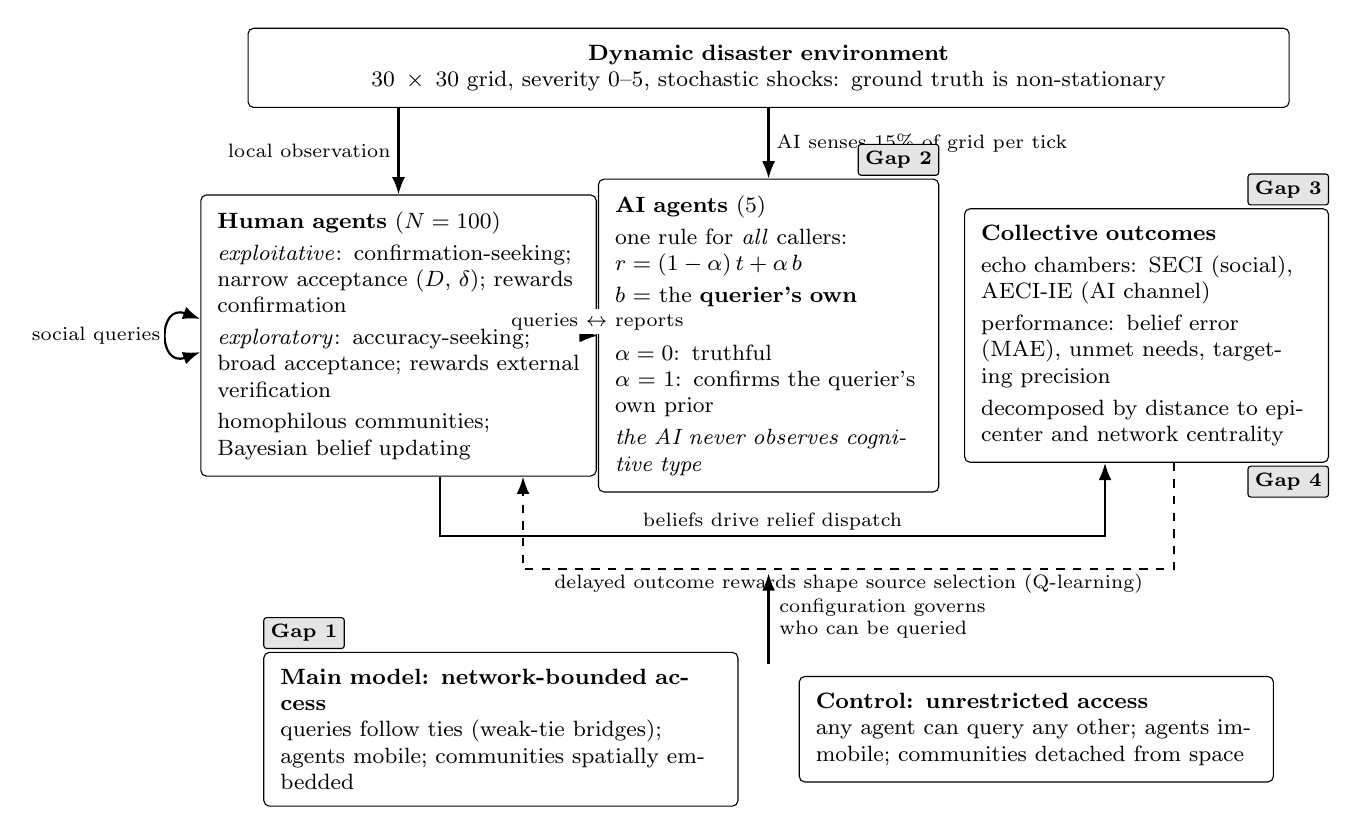
\begin{tikzpicture}[
  font=\footnotesize,
  box/.style={draw, rounded corners=2pt, align=left, inner sep=6pt},
  gapbadge/.style={draw, rounded corners=1pt, fill=black!10, inner sep=2.5pt, font=\scriptsize\bfseries},
  lab/.style={font=\scriptsize, fill=white, inner sep=1.5pt},
  arr/.style={-{Latex[length=2.2mm]}, thick},
  arrd/.style={-{Latex[length=2.2mm]}, thick, dashed},
  biarr/.style={{Latex[length=2.2mm]}-{Latex[length=2.2mm]}, thick}
]
% ---------- Environment ----------
\node[box, align=center, text width=12.8cm] (env) at (7.0,0)
  {\textbf{Dynamic disaster environment}\\
   $30 \times 30$ grid, severity 0--5, stochastic shocks: ground truth is non-stationary};

% ---------- Actors and outcomes ----------
\node[box, text width=4.6cm] (hum) at (2.3,-3.4)
  {\textbf{Human agents} ($N = 100$)\\[2pt]
   \emph{exploitative}: confirmation-seeking; narrow acceptance ($D$, $\delta$); rewards confirmation\\[2pt]
   \emph{exploratory}: accuracy-seeking; broad acceptance; rewards external verification\\[2pt]
   homophilous communities;\\ Bayesian belief updating};
\node[box, text width=3.9cm] (ai) at (7.0,-3.4)
  {\textbf{AI agents} (5)\\[2pt]
   one rule for \emph{all} callers:\\ $r = (1-\alpha)\,t + \alpha\,b$\\[2pt]
   $b$ = the \textbf{querier's own prior}\\[2pt]
   $\alpha = 0$: truthful\\
   $\alpha = 1$: confirms the querier's own prior\\[2pt]
   \emph{the AI never observes cognitive type}};
\node[box, text width=4.2cm] (out) at (11.8,-3.4)
  {\textbf{Collective outcomes}\\[2pt]
   echo chambers: SECI (social), AECI-IE (AI channel)\\[2pt]
   performance: belief error (MAE), unmet needs, targeting precision\\[2pt]
   decomposed by distance to epicenter and network centrality};

% ---------- Environment to actors ----------
\draw[arr] (env.south -| hum.north) -- node[lab, left=1pt]{local observation} (hum.north);
\draw[arr] (env.south -| ai.north)  -- node[lab, right=1pt]{AI senses 15\% of grid per tick} (ai.north);

% ---------- Query channels ----------
\draw[biarr] (hum.east |- ai.west) -- node[lab, above]{queries $\leftrightarrow$ reports} (ai.west);
\draw[biarr] ([yshift=6pt]hum.west) to[out=160, in=200, looseness=3.5]
  node[lab, left=1pt]{social queries} ([yshift=-6pt]hum.west);

% ---------- Beliefs to decisions and feedback ----------
\coordinate (fwd1) at ([xshift=15pt]hum.south);
\coordinate (fwd2) at ([xshift=-15pt]out.south);
\draw[arr]  (fwd1) -- ++(0,-0.75) -| node[lab, above, pos=0.25]{beliefs drive relief dispatch} (fwd2);
\coordinate (fb2) at ([xshift=45pt]hum.south);
\draw[arrd] ([xshift=25pt]fwd2) -- ++(0,-1.35) -|
  node[lab, below, pos=0.25]{delayed outcome rewards shape source selection (Q-learning)} (fb2);

% ---------- Configurations ----------
\node[box, text width=5.6cm] (main) at (3.6,-8.4)
  {\textbf{Main model: network-bounded access}\\ queries follow ties (weak-tie bridges); agents mobile; communities spatially embedded};
\node[box, text width=5.6cm] (ctrl) at (10.4,-8.4)
  {\textbf{Control: unrestricted access}\\ any agent can query any other; agents immobile; communities detached from space};
\coordinate (cmid) at ($(main.north east)!0.5!(ctrl.north west)$);
\draw[arr] (cmid) -- node[lab, right=2pt, align=left]{configuration governs\\ who can be queried} ++(0,1.15);

% ---------- Gap badges ----------
\node[gapbadge, anchor=south west] at ([yshift=1pt]main.north west) {Gap 1};
\node[gapbadge, anchor=south east] at ([yshift=1pt]ai.north east)   {Gap 2};
\node[gapbadge, anchor=south east] at ([yshift=1pt]out.north east)  {Gap 3};
\node[gapbadge, anchor=north east] at ([yshift=-1pt]out.south east) {Gap 4};
\end{tikzpicture}}
\caption{The model and its mapping to the research gaps. A non-stationary disaster environment is observed locally by 100 human agents of two cognitive types and partially sensed by five AI agents. Humans query social contacts or the AI, which answers \emph{every} caller with the same rule, interpolating between truth and the querier's own prior via $\alpha$ (Gap~2, Sec.~\ref{sec:claim2}); the AI never observes a caller's cognitive type, so all type differences arise from human acceptance, evaluation and reward. Agents act on the resulting beliefs by dispatching relief, and delayed outcome rewards feed back into source selection. Which contacts can be queried is governed by the configuration: the main model bounds access by a spatially embedded network with mobility, the control leaves access unrestricted (Gap~1, Sec.~\ref{sec:claim1}). Outcomes are measured at community and population level (Gap~3, Sec.~\ref{sec:claim3}) and decomposed by position in space and network (Gap~4, Sec.~\ref{sec:claim4}). Full specification in Materials and Methods; parameters in Supplementary Table~S1.}\label{fig:concept}
\end{figure}

\section{Results}\label{sec:results}

Throughout, $\alpha$ is swept over eleven levels ($0.0, 0.1, \ldots, 1.0$) with $N = 20$ replications per level, every sweep run under both configurations on identical seeds so that replicates can be compared pairwise. Steady-state values are means over the last 75 of 200 ticks; an effect is called seed-robust only when the paired per-seed confidence interval excludes zero.

Two echo-chamber indices carry the argument, and they share one construct. Echo chambers are a loss of belief diversity: a group whose members hold markedly more homogeneous beliefs than the surrounding population is epistemically insular. The \emph{Social Echo Chamber Index} (SECI) compares belief variance within each social community to the population's belief variance, restricted to beliefs about disaster-affected cells so that agreement on the uninformative `no impact' majority cannot mask insularity. Its AI-side counterpart, the \emph{information-environment index} AECI-IE, applies the identical variance ratio, normalization and filter to the \emph{report levels a channel serves} a community's members --- so that the pair measures the same thing on the two channels through which beliefs are supplied. Negative values indicate an echo chamber for both. A human-channel version, SECI-IE, serves as a consistency check, and AECI-IE-rel compares the served pool against the community's \emph{own} beliefs, distinguishing a channel that narrows what a community sees from one that merely mirrors it back (Materials and Methods; Supplementary Table~S2). Because variance-based indices cannot distinguish convergence on truth from convergence on error, they are read throughout alongside the belief error (MAE) over affected cells and two operational measures: \emph{unmet needs}, the number of high-need cells (severity $\geq 3$) receiving no relief in a tick, and \emph{targeting precision}, the share of relief tokens placed on high-need cells.

\subsection{Network-bounded access is the structural precondition}\label{sec:claim1}

Whether AI can build or break community echo chambers depends first on the structure of information access --- the condition Gap~1 identified as untested. Reported per agent type, the two configurations diverge sharply at high alignment (Fig.~\ref{fig:comparison}a,b). Under unrestricted access, high alignment \emph{dissolves} the confirmation-seekers' echo chamber: SECI for exploitative communities rises to approximately $+0.02$ at $\alpha \geq 0.9$, from $-0.24$ at the truthful endpoint. Under network-gated access the same chamber persists, at $-0.27$ and $-0.31$ at $\alpha = 0.9$ and $1.0$. The paired per-seed difference is large and seed-robust: $\Delta \text{SECI}_{\text{exploit}} = -0.293$ and $-0.338$ at $\alpha = 0.9$ and $1.0$ (main $-$ control, 95\% CI excluding zero; Supplementary Table~S1).

The accuracy-seekers behave differently, and the contrast is instructive. Their communities deepen with alignment in \emph{both} configurations ($-0.01 \rightarrow -0.33$ main; $+0.01 \rightarrow -0.30$ control), so the $\alpha$-gradient of any combined index is explorer-driven everywhere, while the configuration contrast is exploiter-driven. Reporting SECI per type is therefore not a refinement but a requirement: the combined index conceals two mechanisms that run on different axes.

The mechanism is one of exposure, not of targeting. A confirming AI supplies each caller a narrowed version of what that caller already believes. Whether this compounds into \emph{community}-level insularity depends on what else the caller hears. Under unrestricted access roughly half of human queries reach agents outside the caller's community, so out-group beliefs continuously perturb the community's consensus and the confirming signal cannot accumulate; under network-gated access communities are epistemically closed but for sparse weak-tie bridges, and nothing erodes the individually confirmed beliefs into which members settle. Bounded access is thus required for a confirming AI to \emph{preserve} a community chamber --- it does not create one. Consistent with this reading, an ablation in which the AI instead targets the caller's trusted-network consensus leaves every headline result statistically unchanged (Supplementary Table~S4): the amplification does not depend on the AI knowing anything about a caller beyond that caller's own revealed beliefs.

That strongly negative indices at $\alpha = 0$ do not signal comparable harm is settled by the accuracy metrics: at low alignment, homogeneity coincides with the lowest belief errors of the sweep, so convergence there is convergence on the truth, whereas the deepening at high alignment coincides with the largest errors (Fig.~\ref{fig:comparison}c).

\begin{figure}[h]
\centering
\includegraphics[width=\textwidth]{comparison_configs_pertype.png}
\caption{Configuration comparison across the alignment sweep (mean $\pm$ s.e.m. over $N = 20$ paired replications; steady state, last 75 ticks). \textbf{(a)} SECI for confirmation-seeking (exploitative) communities: the chamber dissolves with alignment under unrestricted access and persists under network-gated access. \textbf{(b)} SECI for accuracy-seeking (exploratory) communities, which deepen in both configurations. \textbf{(c)} Belief error (MAE) per agent type: the accuracy cost of alignment falls on the accuracy-seekers, while the confirmation-seekers' error is flat. \textbf{(d)} Unmet high-need cells per tick. Negative echo-chamber indices indicate a chamber. Blue: control (unrestricted access, immobile agents); orange: main model (network-gated access, mobility, spatially embedded bridged network).}\label{fig:comparison}
\end{figure}

\subsection{Confirming AI harms through starvation, not persuasion}\label{sec:claim2}

Gap~2 asked whether harm rises monotonically with alignment and whether a truthful AI is automatically safest. Neither holds, and the reason is that alignment does not work by changing minds --- it works by withholding information.

The accuracy cost is borne almost entirely by the accuracy-seekers. Explorer belief error degrades monotonically with alignment, from $0.55$ at $\alpha = 0$ to $1.74$--$1.75$ at $\alpha \geq 0.9$ in the main model ($0.62 \rightarrow 1.94$ in the control), while exploiter error is flat at approximately $1.8$ across the entire sweep (Fig.~\ref{fig:comparison}c). Confirmation-seekers are already insulated by their narrow acceptance windows; there is little accuracy left for a confirming AI to take from them. The mechanism on the explorer side is visible in the information they hold at all: their pool of beliefs about affected cells collapses from roughly 114 to 27 per agent between $\alpha = 0$ and $\alpha = 1$ (109 to 18 in the control). A confirming AI echoes their mostly-empty priors about the uncertain cells they deliberately query, so they stop acquiring disaster knowledge altogether. This is belief starvation, and it matters for interpretation: part of the explorer SECI deepening in Sec.~\ref{sec:claim1} is this pool shrinkage rather than convergence on a shared false narrative, which is why the pool is reported alongside SECI throughout (Supplementary Fig.~S2).

The AI-channel index tracks the same asymmetry. For accuracy-seekers, AECI-IE deepens with alignment (\fillnum{explorer AECI-IE, $\alpha=0$} $\rightarrow$ \fillnum{explorer AECI-IE, $\alpha=1$}), and the relative index AECI-IE-rel confirms that the AI serves them a pool markedly narrower than their own belief spread. % Provisional (4-seed, 150-tick zoom, main model): AECI-IE -0.24 -> -0.60; AECI-IE-rel -0.32 -> -0.68. NOT citable; extract N=20 per-type values from results-final/.
For confirmation-seekers the index moves the other way (\fillnum{exploiter AECI-IE, $\alpha=0$} $\rightarrow$ \fillnum{exploiter AECI-IE, $\alpha=1$}), and AECI-IE-rel approaches zero: at full alignment the AI serves these communities precisely their own beliefs back, so it has ceased to be an independent source of information rather than becoming a narrower one. % Provisional (same zoom): AECI-IE -0.49 -> -0.14; AECI-IE-rel -0.43 -> -0.02.
The two readings are one phenomenon seen from two sides --- a channel that supplies nothing the receiver did not already hold --- and the paired configuration contrast on the relative index is seed-robust at the confirming end ($\Delta$AECI-IE-rel $= +0.153$ $[+0.104, +0.201]$ at $\alpha = 0.9$ and $+0.161$ $[+0.116, +0.205]$ at $\alpha = 1.0$).

A manipulation check bounds how the dose should be read. Because reports are delivered as integer severity levels, the fraction of reports that exactly match the caller's prior --- the \emph{delivered} confirmation --- is a step function of nominal $\alpha$: approximately $0.14$ at $\alpha = 0.3$, $0.60$ at $\alpha = 0.5$, $0.81$ at $\alpha = 0.6$, and exactly $1.00$ at $\alpha \geq 0.9$, where $\alpha = 0.9$ and $\alpha = 1.0$ are identical at the level of what is served. The sharp operational transition between $\alpha = 0.8$ and $\alpha = 0.9$ reported below is therefore a saturation boundary of the delivery mechanism, not a threshold in the underlying policy, and nominal $\alpha$ understates confirmation in the mid-range (Supplementary Table~S2).

Because the two chamber mechanisms penalize opposite ends of the alignment axis --- the truthful end through the convergence a shared source induces among its heaviest users, the confirming end through starvation and social insularity --- their sum is minimized in the interior. In the main model, every composite definition places $\alpha^{*}$ strictly inside the sweep, with a spread of $[0.3, 0.6]$ across variants (Fig.~\ref{fig:goldilocks}a). In the control the picture divides: composites built only on echo indices select $\alpha^{*} = 1.0$, because full confirmation dissolves the exploiter chamber there, while composites including belief error remain interior. Interiority is therefore a structural property, and must be stated with that qualifier. The operational side agrees: unmet high-need cells reach their minimum in the mid-range while targeting precision stays flat to $\alpha \approx 0.7$ before declining (Fig.~\ref{fig:comparison}d).

Whether an interior optimum exists at all is a property of the population. In cognitively homogeneous populations with baseline or open acceptance, $\alpha^{*} = 0$ --- a truthful AI, with nothing gained from confirmation (Fig.~\ref{fig:goldilocks}b). The interior optimum emerges only once confirmation-seekers are present, or when the whole population is closed-minded, and $\alpha^{*}$ then rises with both polarization and closedness while open populations keep it at $0.3$--$0.4$ throughout. The cost paid \emph{at the optimum} rises along both axes: populations that require more confirmation to accept information are worse off even under their own best policy.

\begin{figure}[h]
\centering
\includegraphics[width=\textwidth]{goldilocks_pnas.png}
\caption{The alignment optimum. \textbf{(a)} Range-normalized composites versus $\alpha$ in the main model: the bubble composite $|\text{SECI}|_{\text{norm}} + |\text{AECI-IE}|_{\text{norm}}$ and the operational composite adding normalized belief error, with the $\alpha^{*}$ spread band $[0.3, 0.6]$ across composite variants; the control's bubble composite is overlaid, its minimum at the confirming boundary. \textbf{(b)} The optimum as a function of the population's cognitive profile: $\alpha^{*}$ across the cognitive gap $g$ for closed, baseline and open acceptance midpoints ($4 \times 3 \times 11$ conditions, $N = 20$ each, main model). Composites are defined within a single sweep and are never compared across configurations; only $\alpha^{*}$ locations are contrasted. Full sensitivity across composite variants, including the retired variance-based AECI-Var, in Supplementary Table~S2.}\label{fig:goldilocks}
\end{figure}

\subsection{The feedback loop: capture, lock-in, and operational buffering}\label{sec:claim3}

Gap~3 asked how echo chambers propagate through the loop from beliefs to decisions and back. That loop closes differently for the two types, and neither closure is corrective.

Confirmation-seekers are captured. Their share of queries directed to the AI rises monotonically with alignment, from $0.47$ to $0.70$, and their trust in it rises alongside: the source that satisfies their acceptance window is selected more often, which exposes them to more of it. Accuracy-seekers show the complementary failure. They do \emph{not} learn to distrust a confirming AI --- their trust in it stays high across the entire sweep ($0.85 \rightarrow 0.81$ at $\alpha = 1$) --- because verification is base-rate dominated: approximately $90\%$ of queried cells are truly empty, so an AI that echoes mostly-correct `no impact' priors passes external verification on almost everything it says, failing only on the rare high-severity cells that matter. Their beliefs freeze instead: relative to their AI-light peers, AI-heavy explorers' belief mobility declines from $-0.04$ to $-0.16$ with alignment (Supplementary Fig.~S3). The failure of accuracy-seeking under base-rate-dominated verification is a substantive finding, not a limitation of the design; a salience-weighted verification channel, in which errors about disaster cells count more than confirmations of empty ones, is retained as the counterfactual (Supplementary Fig.~S6).

Structure buffers the operational consequences even as it preserves the epistemic ones. At $\alpha \geq 0.9$, unmet high-need cells reach $10.0$--$10.3$ per tick in the control but only $2.5$--$3.1$ in the main model; exploiter targeting precision is $0.22$ against $0.37$, and explorer precision falls to $0.21$ in the control against $0.63$ in the main model. Two mechanisms produce this, and both operate independently of the AI: mobility gives agents first-hand observation coverage that no degree of confirmation can distort, and network-gated querying concentrates social exchange on contacts whose local observations are accurate about the caller's surroundings. Because part of every agent's reward signal stays grounded in observation, source-selection learning keeps receiving corrective evidence.

The comparison therefore reveals a trade-off rather than a uniform benefit of structural realism. The same boundedness that anchors operational performance is what allows a confirming AI to preserve social echo chambers (Sec.~\ref{sec:claim1}). Structural realism shifts the failure mode of sycophantic AI from operational collapse toward epistemic insularity --- a failure that operational dashboards would not show.

\subsection{Harms concentrate on the spatial periphery}\label{sec:claim4}

The fourth finding traces how harm is distributed --- the equity question of Gap~4. In the main model, the belief-error gap between agents spawned in the furthest and nearest quartiles from the epicenter widens monotonically with alignment, from $+0.13$ at $\alpha = 0$ to $+0.32$ at $\alpha = 1$ (Fig.~\ref{fig:periphery}a): agents remote from events, who depend almost entirely on mediated reports, absorb the accuracy loss confirmation produces. The behavioral consequence is withdrawal. Relief contributed by far-spawned agents falls from $16.2$ to $6.2$ tokens per agent per five-tick window across the sweep, a decline of $62\%$, against $18.5$ to $13.4$ ($-28\%$) for near-spawned agents (Fig.~\ref{fig:periphery}b) --- the remote quartile does not merely become less accurate, it largely stops sending assistance.

Network position offers no comparable protection: belief-error differences between high- and low-betweenness agents stay within $0.06$ at every alignment level (Supplementary Table~S3). In the immobile control both gaps are approximately zero at all $\alpha$, as the structural-null design requires. The harms of a confirming AI are thus spatially, not topologically, structured: they fall on those who cannot check reports against first-hand observation, however well connected they are --- precisely the position of the remote coordination hubs that dominate data-driven crisis response \citep{comes2020coordination,coleman2024weaving}.

\begin{figure}[h]
\centering
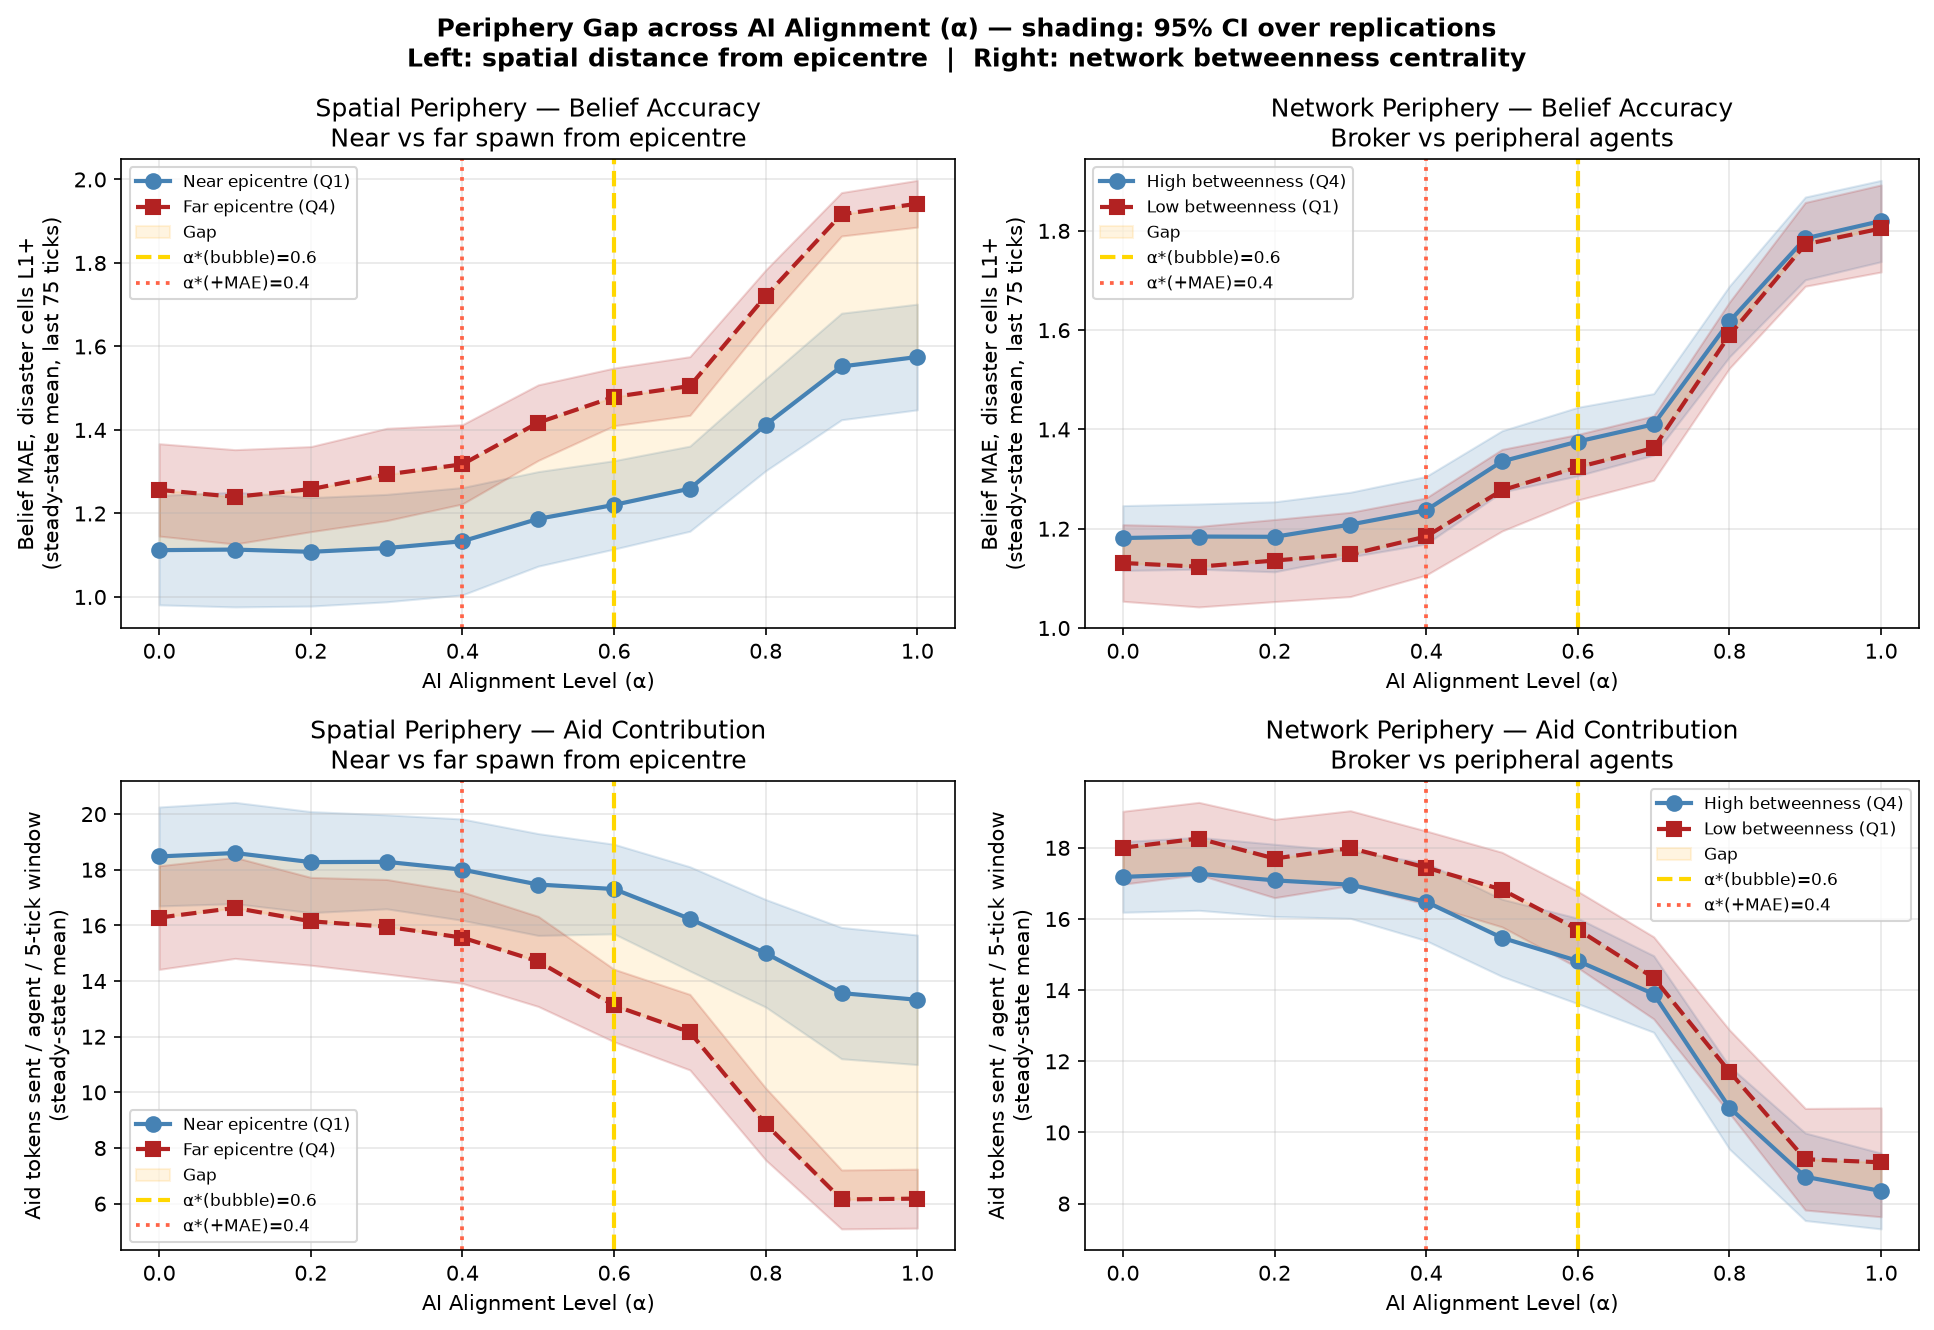
\includegraphics[width=\textwidth]{periphery_gap.png}
\caption{Distribution of alignment harms across space (main model; steady state, last 75 ticks; $N = 20$; bands are 95\% confidence intervals across replications). \textbf{(a)} Belief-error gap between agents spawned in the furthest and the nearest quartile from the epicenter, main model versus control. \textbf{(b)} Relief-contribution gap for the same quartiles. Both gaps are approximately zero at every $\alpha$ in the immobile control, which serves as the structural null. The network-centrality decomposition is in Supplementary Table~S3 and the within-run evolution of both gaps in Supplementary Fig.~S4.}\label{fig:periphery}
\end{figure}

\section{Discussion}\label{sec:discussion}

An AI that pleases its users does not persuade them into error. It withholds, and it is selected for. Confirmation-seekers are \emph{captured}: the source tuned to satisfy their acceptance windows is chosen ever more often, and their community chambers survive wherever the social fabric does not expose them to anything else. Accuracy-seekers are \emph{starved}: the same system answers their deliberately uncertain queries with their own empty priors, their stock of knowledge about the disaster collapses, and the verification channel they rely on cannot catch it because most of what a sycophantic AI says is trivially true. Social structure then decides which failure is visible. Under unrestricted access a confirming AI degrades accuracy and relief while community chambers dissolve; under network-bounded access the same AI leaves relief comparatively intact while chambers persist and deepen.

This extends the experimental literature on human--AI feedback loops from dyads to networks. Dyadic experiments show that interaction with biased AI amplifies individual bias beyond human--human interaction \citep{glickman2024human}. Whether that amplification aggregates into collective echo chambers turns out to be governed by a variable invisible at the dyadic level: who can query whom. This parallels networked collective intelligence, where the effect of social influence on crowd accuracy reverses with structure \citep{lorenz2011social,becker2017network}, and it cautions against extrapolating individual-level sycophancy findings \citep{sharma2024generative} to populations. The control shows what a model without structural constraints would have concluded --- that confirmation weakens echo chambers, with optimal alignment at the confirming boundary. That conclusion is an artifact of unrestricted access, which suggests such models may systematically underestimate the epistemic risks of belief-aligned AI while overestimating its operational risks.

The interior optimum should be read as a descriptive property of a trade-off, \textbf{not} as a design recommendation. Both extremes are dominated in our setting: the truthful end by the convergence a shared source induces among its heaviest users, the confirming end by starvation and its operational consequences. But "build mildly sycophantic AI" does not follow, for two reasons. First, the location of the optimum is a property of the population, not of the technology: the same policy is benign, optimal or harmful depending on the cognitive profile it serves, so no $\alpha^{*}$ transfers across settings. Second, and more fundamentally, confirmation is only one route to adoption. The mechanisms that make a system usable without distorting it --- communicating uncertainty rather than asserting extrapolations with unearned confidence, exposing what the system has and has not observed, and supporting rather than substituting verification --- act on the same acceptance problem without paying in accuracy. Our AI is deliberately overconfident about cells it has never sensed, at every $\alpha$; that design choice, not confirmation, is what makes even the truthful endpoint costly.

Two modeling commitments deserve emphasis. The AI is \emph{type-agnostic}: it responds to every caller with the same rule and never observes a caller's cognitive type, so every difference between types in the Results emerges from human acceptance, evaluation and reward. An ablation in which the AI instead targets the caller's trusted-network consensus --- information no deployed system could observe --- changes no headline result (Supplementary Table~S4). And the two echo indices are one construct applied to two channels, which is what licenses reading them jointly; the earlier variance-over-users construct is retained only for transparency in the sensitivity table, because it cannot by design register a bubble in which each user is served their own prior.

Several limitations bound these conclusions. The alignment mechanism is a reduced form: linear interpolation between truth and confirmation stands in for the drift produced by preference-based training \citep{sharma2024sycophancy} and captures neither the semantics nor the latency and coverage failures of deployed systems; its integer delivery also saturates above $\alpha \approx 0.9$, so the dose should be read through delivered rather than nominal confirmation. The population is small ($N = 100$) and the hazard stylized, chosen to keep network structure interpretable across paired runs. Verification operates through an exogenous situation-report channel with fixed delay and noise. The cognitive-gap sweep shows both the existence and the location of the optimum to be properties of the population's cognitive profile --- a caveat against transferring any specific $\alpha^{*}$. Finally, a single uniform AI policy is applied to the whole population; heterogeneous or adaptive policies, including one that tunes toward truthfulness for remote users to counteract the periphery gradient, are a natural extension.

The disaster case supplies concrete stakes, but it is chosen as an extreme case. The mechanisms rest on features many urgent decision situations share: high stakes under time pressure, a non-stationary ground truth, delayed and noisy verification, and access bounded by ties and position \citep{svenson1993time,mendonca2001decision,holguin2012unique}. Public-health emergencies, financial contagion and security operations combine the same ingredients, and we expect the qualitative pattern --- structural boundedness as the switch between operational and epistemic failure, and an interior optimum --- to carry over, while $\alpha^{*}$ and the operational metrics remain domain-specific.

Trustworthy AI is therefore a property of the socio-technical system rather than of the model alone. The identical policy is benign, optimal or harmful depending on the population it serves; and because its most consequential failure is quiet --- deepening insularity behind acceptable-looking dashboards, concentrated on those least able to check --- the alignment level, the network context and the distribution of verification opportunities have to be designed and monitored together.

\section{Materials and Methods}\label{sec:methods}

Full specification, parameter tables and an ODD-protocol description are in the SI Appendix.

\paragraph{Environment and agents.} A $30 \times 30$ grid carries severity levels 0 (no impact) to 5 (critical), initialized as Gaussian decay from a random epicenter; each tick, cells drift toward baseline and receive random shocks (probability $0.10$, magnitude $\pm 2$), so ground truth is non-stationary and information-seeking never terminates. One hundred human agents belong to one of two cognitive types in equal shares. \emph{Exploitative} agents are confirmation-seeking, with a narrow acceptance window ($D = 2.0$) and steep sensitivity ($\delta = 3.5$); \emph{exploratory} agents are accuracy-seeking ($D = 4.0$, $\delta = 1.2$). The types map onto documented individual differences in information processing under uncertainty \citep{hertwig2016homo,march1991exploration}. Both are organized into type-homogeneous communities; in the main model these are anchored to grid centroids with within-community edge probability $0.5$ and independent weak-tie bridges (probability $0.15$ per agent) crossing communities \citep{granovetter1973strength}, while in the control they are disconnected components independent of position. Mobility follows the returner--explorer dichotomy \citep{pappalardo2015returners}: exploitative agents random-walk within a home radius, exploratory agents step toward their most uncertain cell. Sensing radius is zero, so movement alone determines direct-observation coverage --- which is what makes spatial periphery effects structurally possible.

\paragraph{AI reports and alignment.} Five AI agents each sense $15\%$ of the grid per tick with constant noise, independent of $\alpha$. A queried AI answers with
\begin{equation}
r_{\text{AI}} = (1 - \alpha)\, t + \alpha\, b,
\label{eq:alignment}
\end{equation}
where $t$ is the severity as available to the AI and $b$ is \textbf{the querying agent's own current belief, identically for both agent types}. For cells it has not sensed the AI answers with an inverse-distance interpolation or a position-based prior, delivered with the same confidence as sensed values: even at $\alpha = 0$ the AI is truthful only about what it has observed, and this overconfidence applies at every $\alpha$. Reports are delivered as integer levels, so the delivered confirmation fraction is a step function of $\alpha$ that saturates at $\alpha \geq 0.9$; it is recorded in every run as a manipulation check. The AI does not learn, so all learning dynamics are attributable to human agents.

\paragraph{Belief revision and source selection.} A report at distance $d = |r - b|$ from the current belief is accepted with probability $D_{\text{eff}}^{\delta} / (d^{\delta} + D_{\text{eff}}^{\delta})$, where $D_{\text{eff}}$ is trust-widened for friends; accepted reports enter a precision-weighted posterior, generalizing bounded-confidence dynamics \citep{deffuant2000mixing} by replacing a hard threshold with a smooth curve. Agents choose among querying a contact, querying the AI, or acting, by $\epsilon$-greedy Q-learning ($\epsilon = 0.3$, $\eta = 0.10$). The reachable pool is the configuration switch: trust-weighted over all agents in the control, over friends only (with a $0.1$ chance of a two-hop draw) in the main model. Rewards arrive on two timescales --- delayed outcome feedback (15--25 ticks) when relief is processed, and information-quality feedback when reports can be evaluated. The evaluation channel differs by type: exploitative agents score reports for \emph{confirmation} against their own stored prior, exploratory agents for \emph{accuracy} against an exogenous situation-report channel (minimum 3-tick lag, per-tick arrival probability $0.3$, same noise as direct sensing). Reports never verified before a 30-tick expiry produce no learning signal --- explorers do not fall back on their own priors, which would collapse the accuracy channel into a confirmation channel.

\paragraph{Metrics.} All echo indices share a sign convention: negative indicates a chamber, zero is the null. For each community $c$, pooling member beliefs with level $\geq 1$,
\begin{equation}
\text{SECI}_c =
\begin{cases}
(\text{Var}_c - \text{Var}_{\text{glob}})/\text{Var}_{\text{glob}} & \text{Var}_c < \text{Var}_{\text{glob}}, \\[1ex]
(\text{Var}_c - \text{Var}_{\text{glob}})/(5 - \text{Var}_{\text{glob}}) & \text{otherwise},
\end{cases}
\label{eq:seci}
\end{equation}
bounding the index to $[-1, 1]$; values are averaged within each agent type and computed every five ticks \citep{cinelli2021echo}. \textbf{AECI-IE} applies Eq.~\ref{eq:seci} unchanged --- same normalization, same level $\geq 1$ filter, same per-community pooling and per-type averaging --- to the \emph{levels of the reports AI agents deliver} to a community's members during each window, in place of their beliefs; \textbf{SECI-IE} is the same over human-delivered reports and serves as a consistency check against SECI. \textbf{AECI-IE-rel} replaces the global denominator with the community's own belief variance, so that zero marks a channel that mirrors a community's beliefs back and negative values a channel that narrows them; it disambiguates the two ways a served pool can lose diversity. Because a shrinking pool can itself read as homogeneity, the number of level $\geq 1$ reports and beliefs is reported alongside every index. Belief error (MAE) is the mean absolute deviation from true severity over affected cells; relief performance is unmet needs and targeting precision as defined above. Two composites over the steady-state window locate the optimum, range-normalized within a sweep: $|\text{SECI}|_{\text{norm}} + |\text{AECI-IE}|_{\text{norm}}$ and the same plus $\text{MAE}_{\text{norm}}$. Because normalization can amplify a component with a small raw signal, $\alpha^{*}$ is reported as a spread across composite variants, and interiority is additionally tested without normalization through paired per-seed contrasts of the raw composite (Supplementary Table~S2).

\paragraph{Design and analysis.} The primary experiment sweeps eleven $\alpha$ levels with $N = 20$ replications, under both configurations, for 200 ticks. Replicate $i$ uses seed $i$ in every condition, so replicates are paired by seed across $\alpha$ levels and configurations (common random numbers); configurations are compared on \emph{raw} metrics through paired per-seed deltas. Range-normalized composites are defined within a single sweep and never compared across configurations --- only $\alpha^{*}$ locations are contrasted. Per outcome, effects are estimated with mixed-effects models with seed as grouping factor and Holm-corrected per-level contrasts (Supplementary Tables~S1 and~S6). A secondary experiment varies the cognitive gap $g$ and acceptance midpoint $d_{\text{mid}}$ under the main model. The model is implemented in Python 3.11 with Mesa and NetworkX; all runs are seeded and reproduce bit-for-bit within the pinned environment. Figures are regenerated from serialized results without re-simulation.

\backmatter

\bmhead{Supplementary information}
The SI Appendix contains the ODD-protocol model description, parameter and calibration tables, metric definitions, Figs.~S1--S6 and Tables~S1--S10.

\bmhead{Acknowledgements}
%% To be completed.

\section*{Declarations}

\bmhead{Funding} No funding sources provided support for this project.
\bmhead{Conflict of interest} The author declares no competing interests.
\bmhead{Data availability} All simulation outputs underlying the figures and tables are archived with the code repository.
\bmhead{Code availability} The full model, parameter files and post-processing scripts are available at \url{https://github.com/tinacomes/DisasterAI}.

%% All cited keys resolve from References.bib (audit 2026-08-18); one
%% placeholder remains flagged inside References.bib:
%% steinbrink2024transparency.
\bibliography{References}

\end{document}
